\documentclass[11pt,a4paper]{article}
\usepackage[margin=21mm,headheight=14pt]{geometry}
\usepackage[T1]{fontenc}
\usepackage{lmodern,amsmath,amssymb,amsthm,booktabs,array,tabularx,longtable,graphicx,xcolor,fancyhdr,hyperref}
\definecolor{ink}{HTML}{16394D}
\hypersetup{colorlinks=true,linkcolor=ink,citecolor=ink,urlcolor=ink,pdftitle={Noncollision Facet Transition and Exact Outer-Envelope Classification in the Folded Tri-Octagon},pdfauthor={Hilmir Frímann Halldórsson},pdfsubject={Research edition v0.1; project-internal manuscript review complete; author-authorized for repository publication; not externally peer reviewed.},pdfkeywords={Tri-Octagon, convex hull, noncollision facet transition, exact classification}}
\pagestyle{fancy}\fancyhf{}\lhead{\small Folded Tri-Octagon: outer envelopes}\rhead{\small Research edition v0.1}\cfoot{\thepage}
\setlength{\parindent}{0pt}\setlength{\parskip}{5pt}
\setlength{\emergencystretch}{2em}
\newcommand{\xs}{x_*}
\newcommand{\conv}{\operatorname{conv}}
\newcommand{\br}[1]{\textnormal{\texttt{#1}}}
\newcommand{\src}[1]{\par\smallskip{\footnotesize\color{ink}Source: #1\par}}
\newcommand{\cycle}[1]{\texttt{(#1)}}
\newcommand{\rep}[4]{\textbf{#1}\newline #2 faces & $\begin{aligned}#3\end{aligned}$\par\vspace{2pt}{\small Cycle: #4}\\[6pt]}
\theoremstyle{definition}
\newtheorem{theorem}{Theorem}
\newtheorem{proposition}[theorem]{Proposition}
\newtheorem{lemma}[theorem]{Lemma}
\newtheorem{corollary}[theorem]{Corollary}
\begin{document}
\thispagestyle{plain}
{\LARGE\bfseries\color{ink}Noncollision Facet Transition and Exact Outer-Envelope Classification in the Folded Tri-Octagon\par}
\vspace{6pt}
{\small\itshape A companion to Spherical Edge Extensions of the Folded Tri-Octagon: Exact Incidence Events, Natural Terminations, and Convex Envelopes\par}
\vspace{7pt}
{\large Hilmir Frímann Halldórsson}\par
Research edition v0.1 \quad 14 November 2026\par
\vspace{3pt}
{\footnotesize Project-internal manuscript review complete; author-authorized for repository publication.\par
Project-internal research edition, not externally peer reviewed.}
\begin{abstract}
The existing folded Tri-Octagon determines 21 supporting lines and 42 signed exits on a concentric observer sphere. We study their explicitly declared convex envelope across the closed interval from Crossing A to Crossing B. The accepted coincidence catalogue fixes the endpoint mergers but does not determine all intervening supporting faces. There is exactly one interior change of the labelled maximal-face lattice: at midpoint-to-exit distance $t=3h$, all 42 vertices remain distinct while six symmetry-related face patches become maximal hexagons. The two open chambers have 56 and 50 facets, and the transition has 44. Each affected patch changes from two triangles and a quadrilateral to one hexagon, then to two quadrilaterals. Exact supporting-plane and polygon-side signs hold throughout each chamber; closure under true ridge adjacency proves that no facet or interior combinatorial transition is omitted. The limiting polygons recover the inherited A/B hulls. The complete closed-interval list has no ten-vertex maximal facet. These are consequences of the fixed exit family and convexification convention, without selecting a physical boundary, preferred observer radius, or dynamical law.
\end{abstract}
\section{Question and contribution}\label{sec:question}
Point coincidence and face reorganization are different geometric events. Distinct exits can enter a common supporting plane without meeting one another. The parent synthesis completely classifies finite line coincidences and the Original, A and B event hulls~\cite{parent}. The present companion supplies the intervening maximal-face classification; it preserves those earlier results.
\par\begin{table}[h]\centering\small
\caption{Accepted contribution boundary. O01 is documentary concordance, not a novelty theorem.}\label{tab:claims}
\begin{tabularx}{\linewidth}{@{}lX@{}}\toprule
Record & Role in this companion\\\midrule
O01 & Bounded source comparison; no earlier interval theorem in the inspected project sources.\\
O02 & Exact noncollision supporting-face event and its six-member orbit.\\
O03 & Complete closed A--B face lattice and attachment to inherited endpoints.\\
O04 & Local regrouping and the scoped absence of ten-vertex maximal facets.\\\bottomrule
\end{tabularx}
\src{Accepted claim ledger and internal review, Section 2~\cite{investigation,review}.}
\end{table}\par

\clearpage
\section{Frozen geometry and the observation family}\label{sec:geometry}
The coordinate authority is Paper C, Section 4~\cite{paperC}. Its centred material vertices $v_0,\ldots,v_{17}$ and three welded octagonal cycles are unchanged. Let $w>0$ be the panel flat-to-flat width and define
\begin{equation}\label{eq:parameters}
h=\frac{\sqrt2-1}{2}w,\qquad x=t/w,\qquad
A=\frac12,\quad B=\frac{1+\sqrt2}{2},\quad
\xs=\frac{3(\sqrt2-1)}2.
\end{equation}
A and B are dimensionless endpoint parameters, not sphere radii. The accepted records call the transition parameter $T$; this manuscript uses $\xs$ throughout. It has no connection to the historical scalar notation $T=\pi e\phi$.

E01--E21 are the lexicographically ordered undirected material endpoint pairs. For an edge with $i<j$, its positive unit direction follows $v_i$ to $v_j$:
\begin{equation}\label{eq:family}
\begin{split}
m_e&=(v_i+v_j)/2,\qquad u_e=(v_j-v_i)/(2h),\\
p_{e,\pm}(x)&=m_e/w\pm xu_e,\qquad
H(x)=\conv\{p_{e,\pm}(x):1\le e\le21\}.
\end{split}
\end{equation}
Here $p$ is a dimensionless position in the physical centred frame. All 42 labels remain in the incidence record, including at A and B where they occupy only 18 positions. $H$ denotes their mathematical convex envelope; it is distinct from the original open three-panel shell and from its supporting-line framework.

The inherited midpoint identities are
\begin{equation}\label{eq:sphere}
|u_e|=1,\quad m_e\cdot u_e=0,\quad |m_e|^2=w^2/3,
\qquad |p_{e,\pm}(x)|^2=1/3+x^2=(R/w)^2.
\end{equation}
The complete coincidence theorem gives 42 distinct positions for every $A<x<B$~\cite[Sections 4--6]{parent}. The common-sphere argument exposes each distinct point: $p\cdot q\le (R/w)^2$, with equality only at $q=p$. Thus these positions are precisely the hull vertices. Full dimension follows from three noncollinear seam exits at height $-x$ and one at $+x$; their tetrahedron has nonzero volume for $x>0$. These facts and the full finite $D_{3h}$ symmetry are inherited premises, not new discoveries.

\subsection{A calculation chart, not an isometry}\label{sec:chart}
The accepted calculation uses the invertible chart
\begin{equation}\label{eq:chart}
(X,Y,Z)=(p_x,p_y/\sqrt3,p_z),\qquad
|p|^2=X^2+3Y^2+Z^2.
\end{equation}
Its positive determinant preserves convexity, support, incidence and cyclic polygon order. It does not preserve Euclidean lengths or angles under the unweighted norm. All affine coefficients in this chart belong to $K=\mathbb Q(\sqrt2)$. The appendix uses charted plane coefficients; the concrete plane in Section~\ref{sec:event} uses physical-frame coefficients.

The certificate stores $a+b\sqrt2$ as the pair $[a,b]$ of rational strings. Polynomial arrays ascend in powers of $x$; an empty array means the zero polynomial. Source vertex, midpoint, direction and branch identities were matched exactly in the accepted investigation~\cite[Sections 1--2]{investigation}. The original minimum ball, endpoint hulls and silver-ratio relation remain inherited background~\cite{parent}; none is re-derived as a new result here.

\clearpage
\section{A supporting-face event without point coincidence}\label{sec:event}
Put $h_1=h/w$. In dimensionless physical coordinates consider
\begin{align}
n(x)&=\left(0,-1,\frac{\sqrt3}{2}(x-h_1)\right),\label{eq:candidate-n}\\
d(x)&=\frac{\sqrt6}{4}x^2+\frac{\sqrt6-\sqrt3}{4}x
       +\frac{\sqrt3}{24}+\frac{\sqrt6}{16}.\label{eq:candidate-d}
\end{align}
For \br{E05+}, \br{E09+}, \br{E17+} and \br{E16-}, the residual $n(x)\cdot p-d(x)$ vanishes identically. For each of \br{E21+} and \br{E10-}, it is
\begin{equation}\label{eq:factor}
r(x)=-\frac{\sqrt6}{4}(x-\xs)(x-B).
\end{equation}
It is negative on $(A,\xs)$ and positive on $(\xs,B)$. The four-label plane is supporting in the first chamber and fails to support the full set in the second. The sign reversal alone is not a completeness proof.

\begin{proposition}[Accepted noncollision event]\label{prop:event}
The parameter $\xs$ lies strictly inside $(A,B)$ and gives a maximal supporting hexagon with outward cyclic order
\begin{equation}\label{eq:hex-cycle}
(\br{E05+},\br{E16-},\br{E21+},\br{E09+},\br{E17+},\br{E10-}).
\end{equation}
Its actual $D_{3h}$ orbit has six facets. All 42 exit positions remain distinct.
\end{proposition}
\begin{proof}
The exact comparisons $3\sqrt2>4$ and $\sqrt2<2$ give $A<\xs<B$. At this parameter,
\[
n_*=(0,-1,\sqrt3h_1),\qquad d_*=-13\sqrt3/12+\sqrt6.
\]
Table~\ref{tab:residuals} gives the complete residual list: precisely the six stated labels are zero and all others are strictly inward. The normal is nonzero. The inherited coincidence theorem excludes any merger here; three distinct points on the common sphere cannot be collinear. The zero set spans a plane, so it is a maximal facet. The accepted strict side tests certify its cyclic order. The coefficient-verified group action gives six distinct image facets, separately from two persistent cap hexagons. No regularity assertion is required.
\end{proof}
\par
\begin{table}[h]\centering\small
\caption{Complete residual classes at $\xs$. Values are $(n_*\cdot p-d_*)/\sqrt3$; every nonzero row is strictly negative.}\label{tab:residuals}
\begin{tabular}{@{}ll@{}}\toprule
Exact residual & Branch labels\\\midrule
$-1 + \frac{\sqrt{2}}{2}$ & \br{E06-}, \br{E08+}, \br{E15-}, \br{E18+} \\
$- \frac{1}{2} + \frac{\sqrt{2}}{4}$ & \br{E07-}, \br{E14+} \\
$- \frac{3}{2} + \frac{\sqrt{2}}{2}$ & \br{E01-}, \br{E02-}, \br{E03-} \\
$1 - \frac{3 \sqrt{2}}{4}$ & \br{E19+}, \br{E19-} \\
$\frac{1}{2} - \frac{\sqrt{2}}{2}$ & \br{E04+}, \br{E11-}, \br{E12+}, \br{E20-} \\
$2 - 2 \sqrt{2}$ & \br{E04-}, \br{E11+}, \br{E12-}, \br{E20+} \\
$3 - \frac{5 \sqrt{2}}{2}$ & \br{E01+}, \br{E02+}, \br{E03+} \\
$3 - \frac{9 \sqrt{2}}{4}$ & \br{E09-}, \br{E17-} \\
$\frac{3}{2} - \frac{3 \sqrt{2}}{2}$ & \br{E05-}, \br{E10+}, \br{E16+}, \br{E21-} \\
$\frac{3}{2} - \frac{5 \sqrt{2}}{4}$ & \br{E13+}, \br{E13-} \\
$\frac{5}{2} - 2 \sqrt{2}$ & \br{E07+}, \br{E14-} \\
$\frac{7}{2} - \frac{5 \sqrt{2}}{2}$ & \br{E06+}, \br{E08-}, \br{E15+}, \br{E18-} \\
$0$ & \br{E05+}, \br{E09+}, \br{E10-}, \br{E16-}, \br{E17+}, \br{E21+} \\
\bottomrule\end{tabular}
\src{Accepted candidate residual table~\cite{investigation}. For example, $(7-5\sqrt2)/2<0$ because $49<50$.}
\end{table}\par


\clearpage
\begin{figure}[p]\centering
{\small\bfseries (a) $x=3/5$: two triangles and one quadrilateral}\par
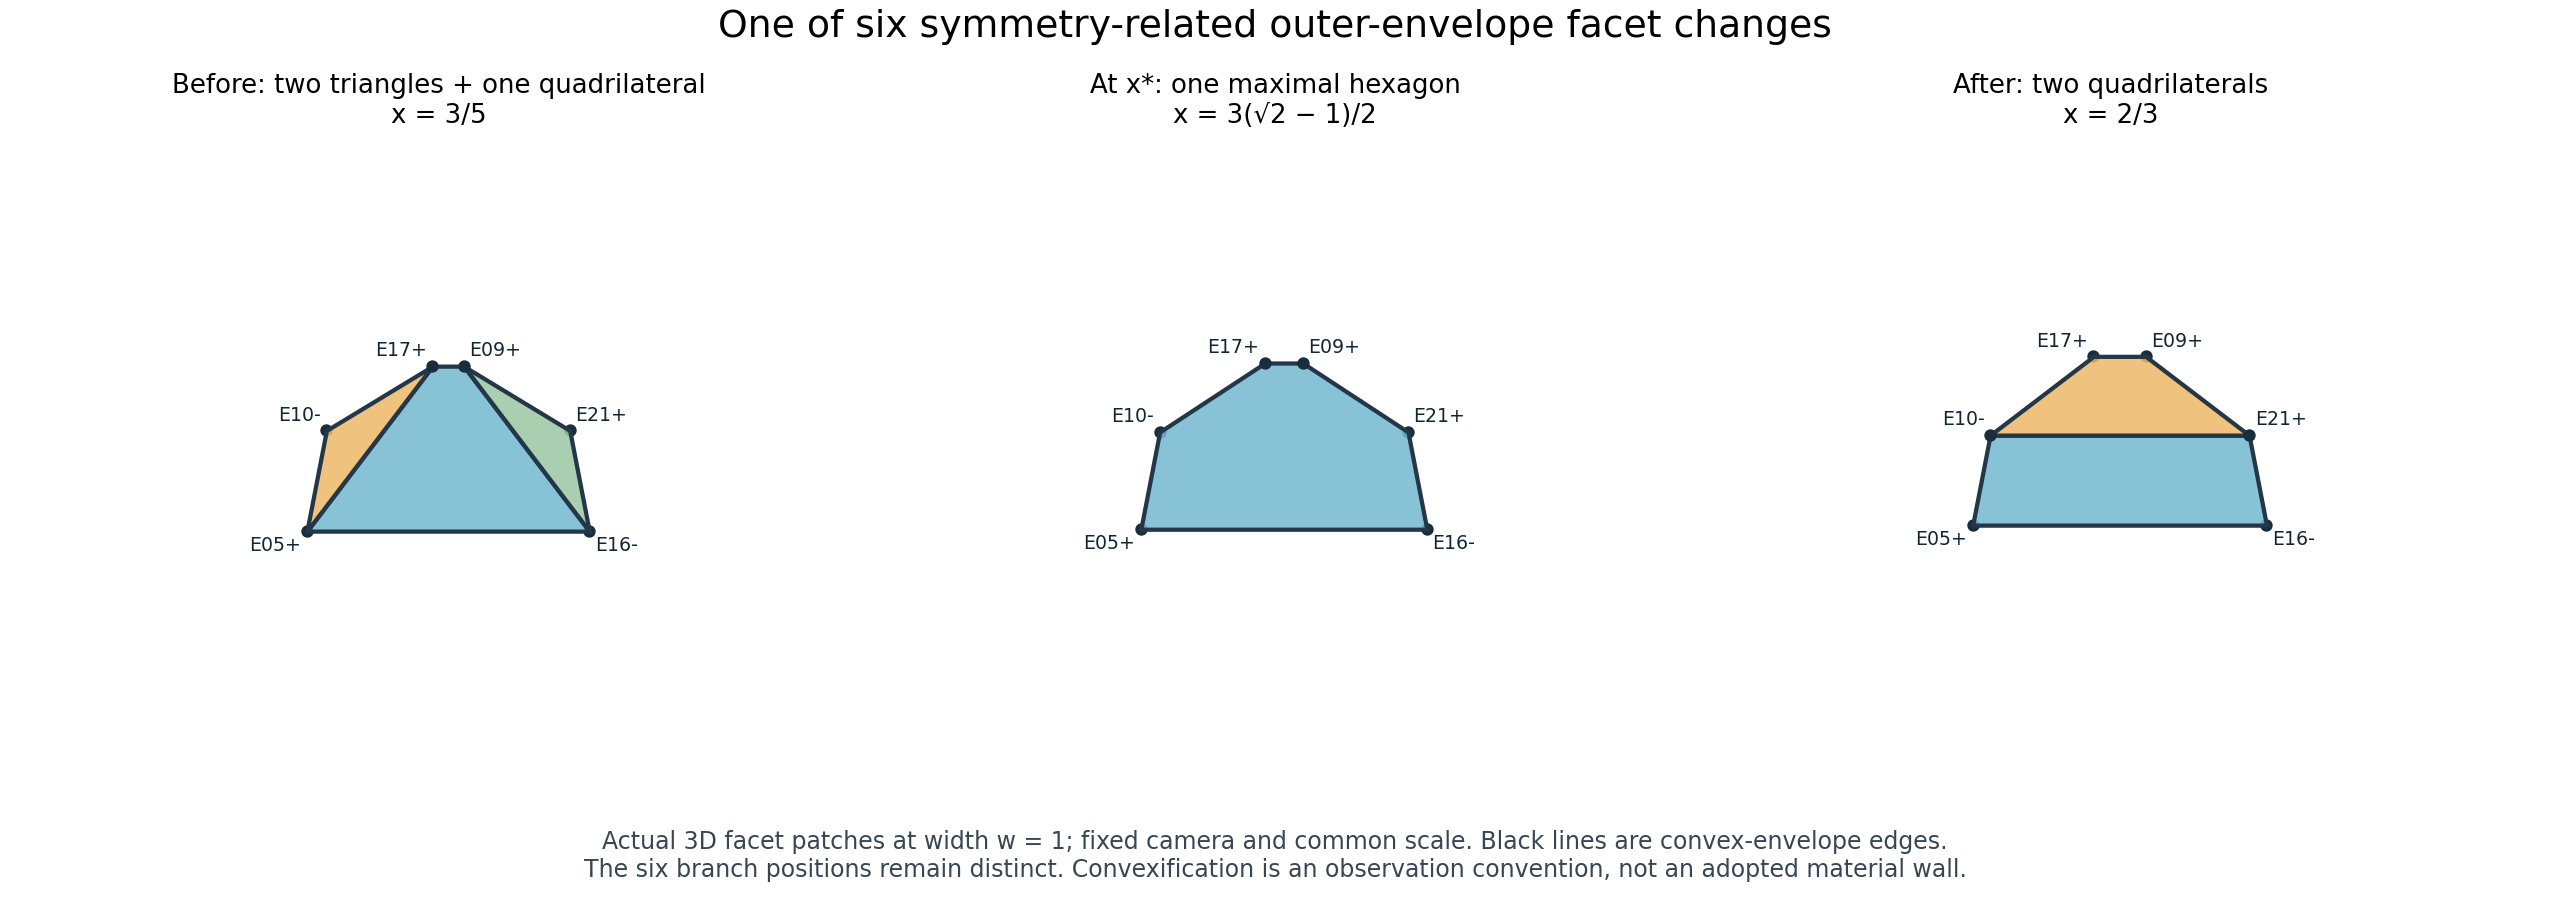
\includegraphics[width=96mm,trim=76.235bp 134.682bp 792bp 127.059bp,clip]{figures/local_facet_transition.png}\par
{\small\bfseries (b) $x=\xs$: one maximal hexagon}\par
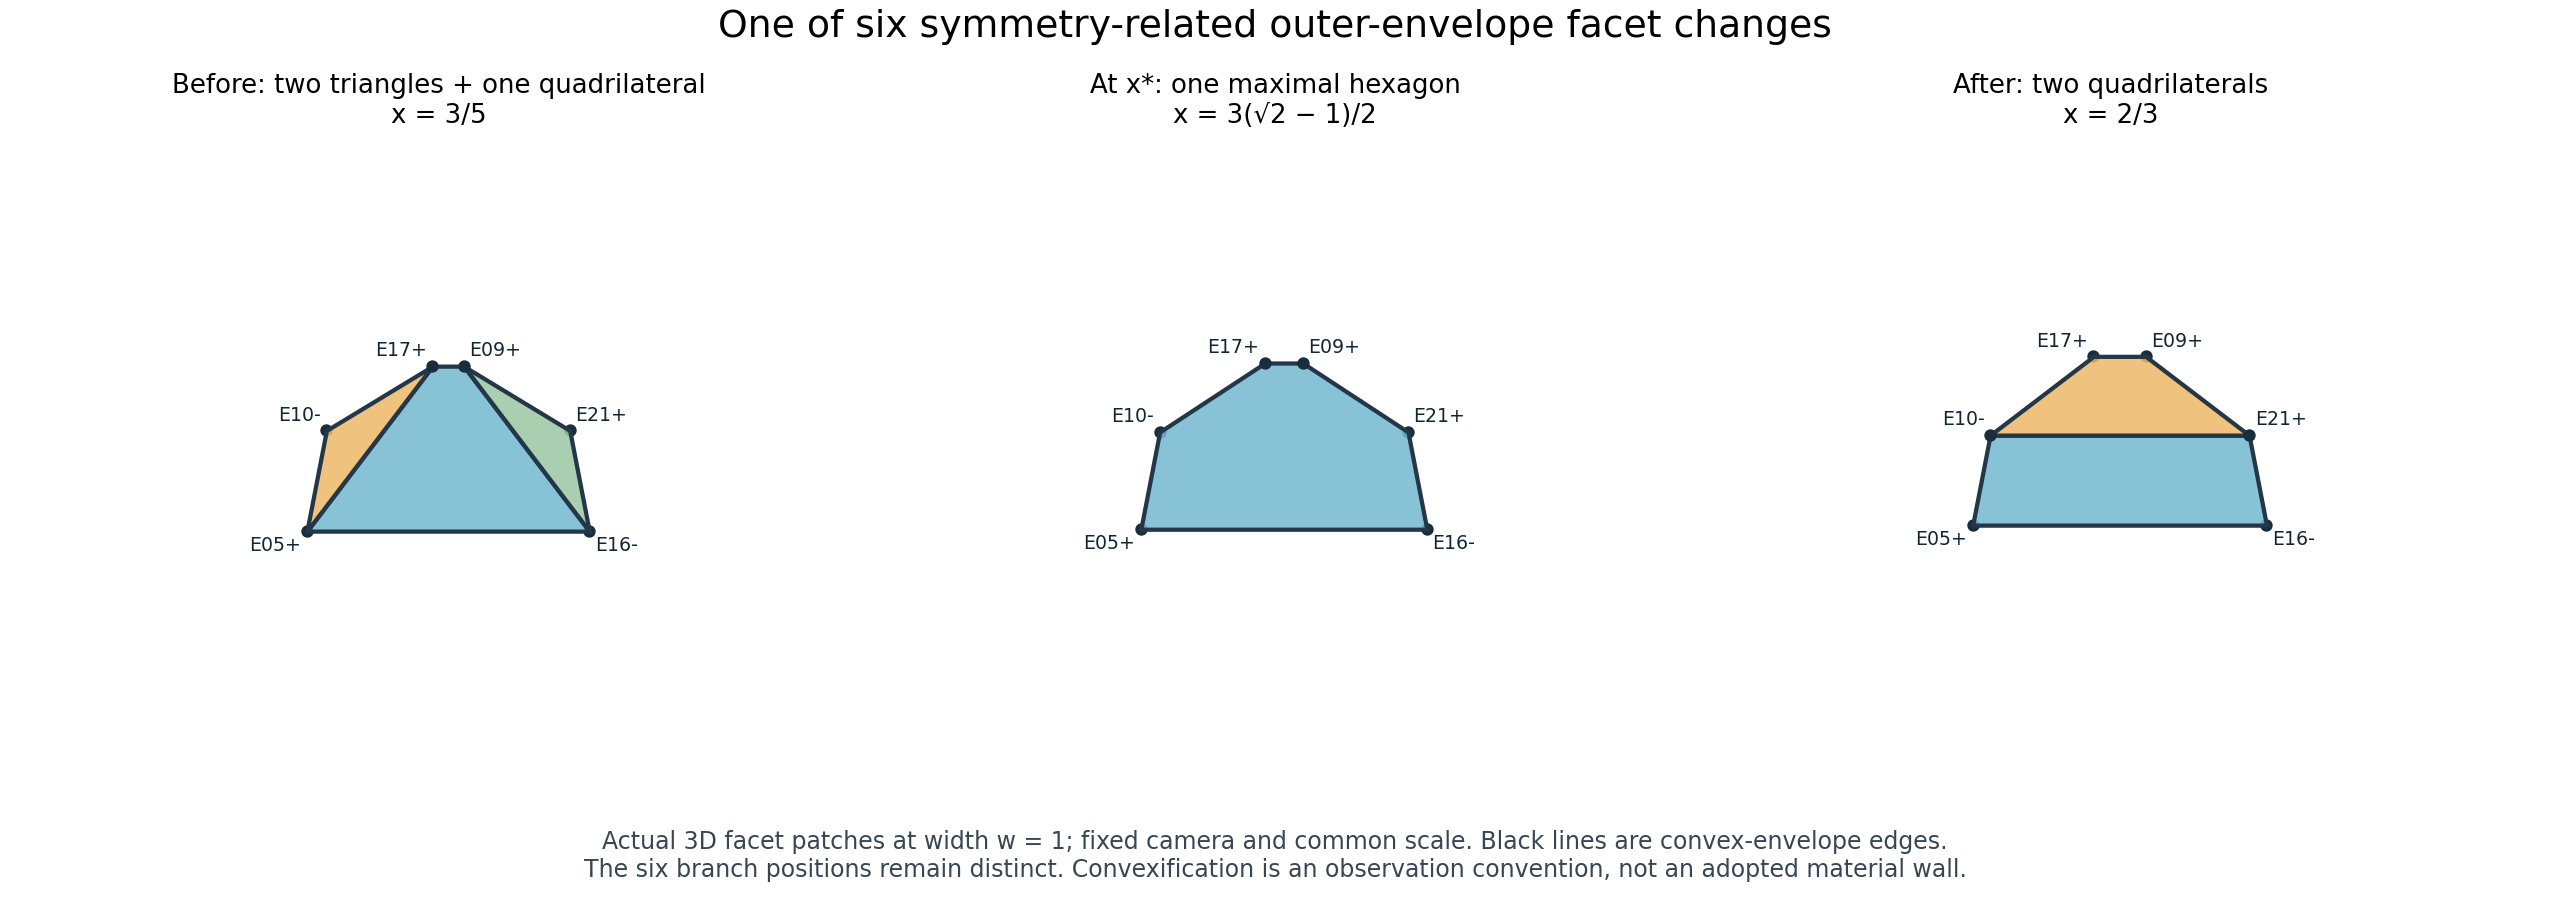
\includegraphics[width=96mm,trim=436.235bp 134.682bp 432bp 127.059bp,clip]{figures/local_facet_transition.png}\par
{\small\bfseries (c) $x=2/3$: two quadrilaterals}\par
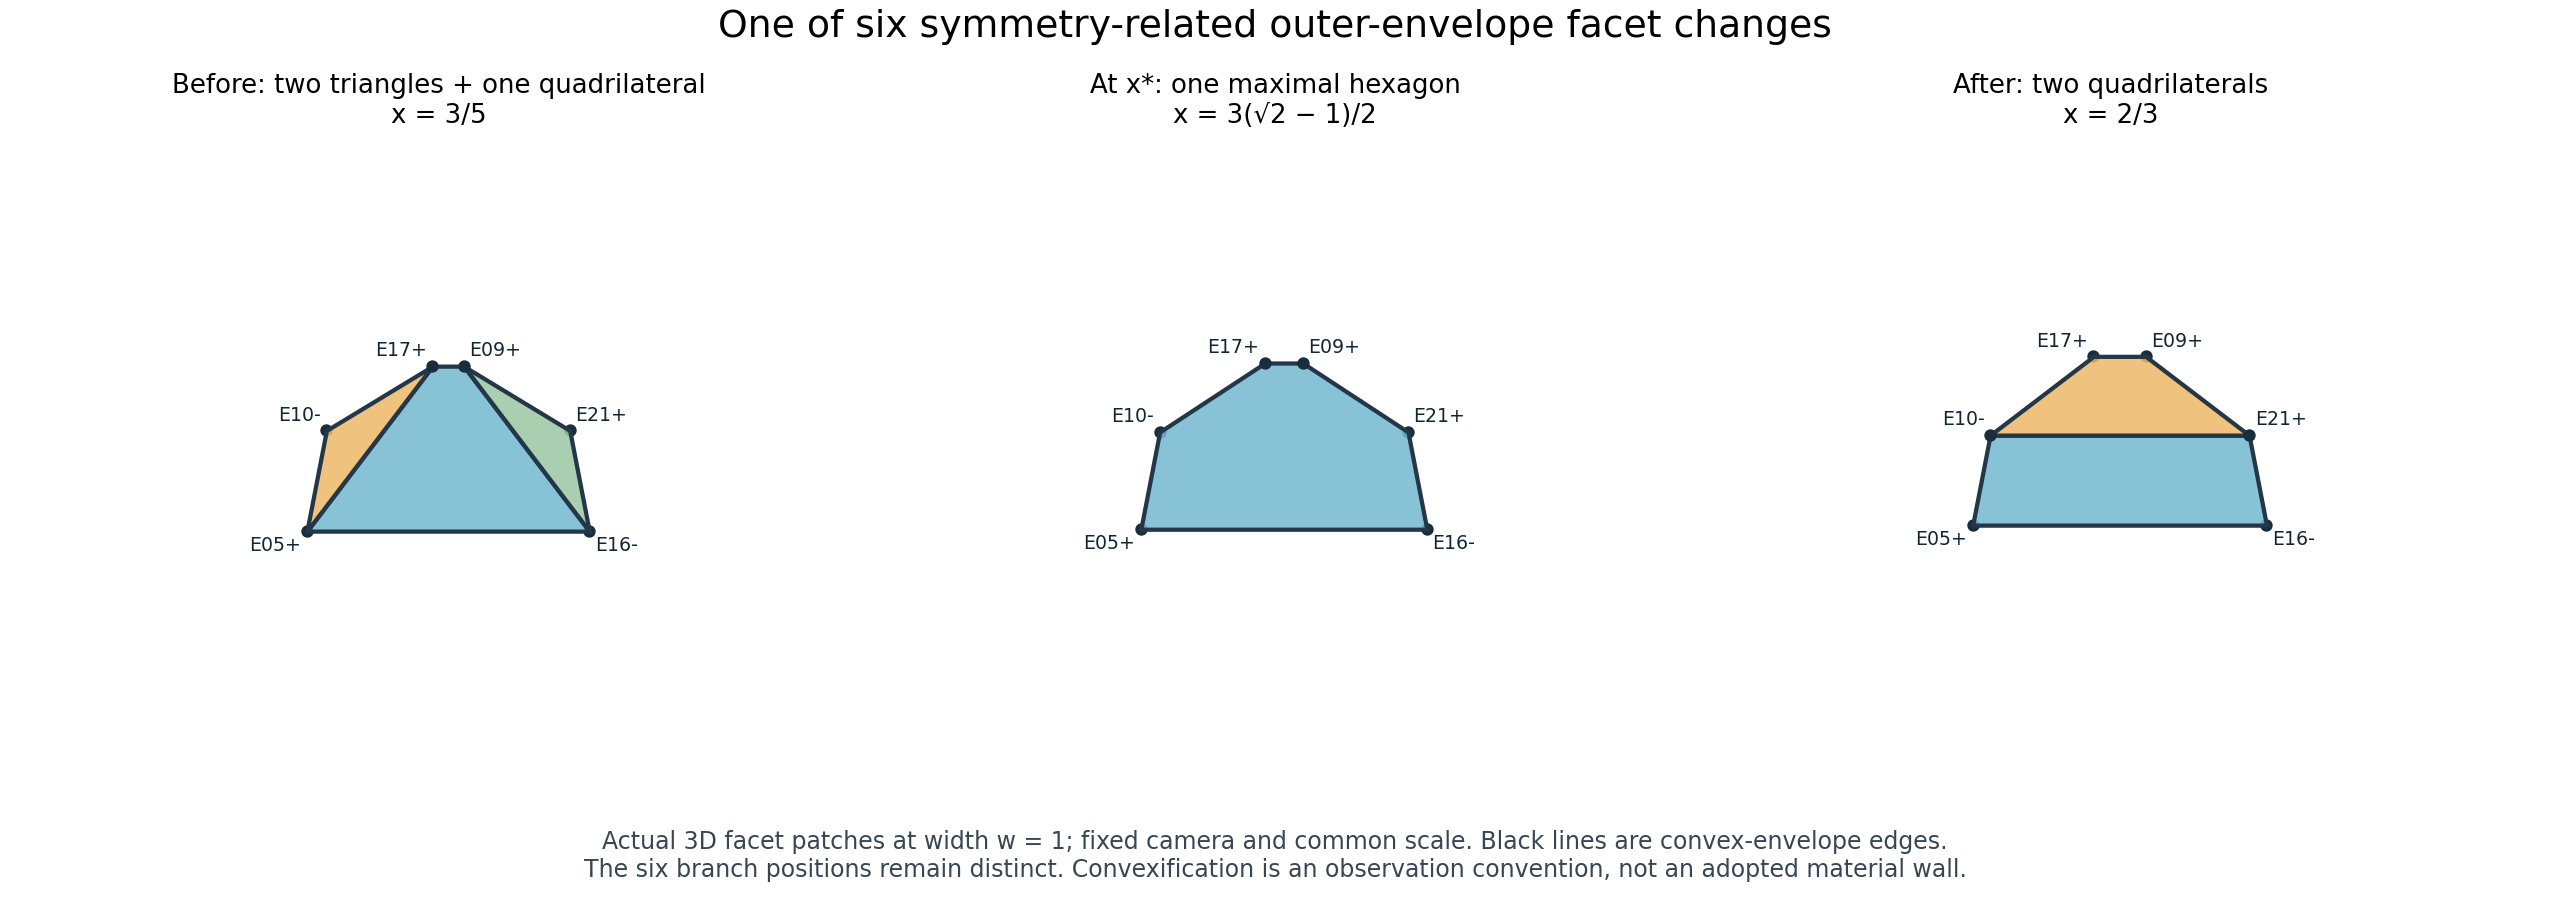
\includegraphics[width=96mm,trim=796.235bp 134.682bp 72bp 127.059bp,clip]{figures/local_facet_transition.png}
\caption{One of six symmetry-related patches, using the accepted illustration. The original three panels are arranged vertically through documentary cropping for label legibility; geometry is unchanged. They use normalized physical coordinates, one camera and a common spatial scale. ``Before'' and ``after'' mean parameter order, not elapsed time. Drawn diagonals are true envelope edges when present, not rewiring of the original supporting lines. Source: investigation figure and transition readout~\cite{investigation}; the unchanged full SVG and PNG remain in the evidence.}\label{fig:transition}
\end{figure}
\clearpage
\section{Exact certificates throughout each chamber}\label{sec:certificates}
The accepted proof validates a finite facet list on each of $(A,\xs)$, $\{\xs\}$ and $(\xs,B)$. Three numerical hulls nominated candidates only. In the calculation chart, a proposed face with first three points $a,b,c$ determines
\begin{equation}\label{eq:face-plane}
N=(b-a)\times(c-a),\qquad D=N\cdot a,\qquad
r_l=N\cdot p_l-D.
\end{equation}
In this section $p_l$ denotes its charted coordinate tuple. Each component of $N$ has degree at most two in $x$; every residual has degree at most three. The accepted conditions are:
\begin{enumerate}
\item $N\cdot N>0$ on the domain, so the proposed plane never degenerates.
\item Exactly the declared facet labels have zero residual. On an open chamber these are identically zero polynomials; every other label has strictly negative residual throughout that chamber.
\item For every directed consecutive side $(a,b)$ and each other face vertex $c$,
\begin{equation}\label{eq:side-test}
N\cdot((b-a)\times(c-a))>0.
\end{equation}
\end{enumerate}
The side polynomials have degree at most four. Their strict signs place every other face vertex inward of each directed side. Consequently the proposed cycle is the genuine convex polygon boundary, rather than a fan of rendering triangles. Complete zero sets merge all coplanar face pieces into their actual maximal polygon. At $\xs$ the same tests are evaluated exactly at the algebraic parameter.

\subsection{Ordered-field signs and open-interval roots}\label{sec:sturm}
For $q=a+b\sqrt2$, the sign is immediate if one summand is zero or the summands have the same sign. If the signs oppose, comparison of the rational quantities $a^2$ and $2b^2$, with the sign of $a$, decides it exactly. Irrationality of $\sqrt2$ excludes equality for nonzero rational $a,b$. Cancellation is therefore handled without a floating tolerance.

For a nonzero polynomial on an open chamber $(l,u)$, the submitted method first divides out every exact factor $x-l$ and $x-u$. Endpoint zeros are permitted and are treated separately at the exceptional parameter. The remaining polynomial has no endpoint root. Its Sturm sequence is constructed by differentiation and negative Euclidean remainders over $K$, using only positive remainder rescalings. The difference in endpoint sign variations counts all distinct interior roots, including even-multiplicity ones. Zero roots together with the required sign at the exact midpoint proves that sign throughout the chamber. Persistent zero polynomials are handled separately; they are not isolated transition candidates.

This gives uniform support, normal and side signs, not a finite-resolution sweep. The complete residual polynomials and cycles are preserved electronically~\cite{investigation}. The 26 plane-orbit representatives in Appendix~\ref{app:planes} provide a compact exact description of every new-domain facet. No all-triples or all-quadruples enumeration is needed for the completeness argument that follows.

\clearpage
\section{Completeness and the closed-interval classification}\label{sec:complete}
\begin{lemma}[Closure under true ridge adjacency]\label{lem:closure}
Let $Q$ be a full-dimensional three-dimensional convex polytope. A nonempty list of its actual maximal facets is complete if every true ridge of each listed facet is incident with two distinct listed facets.
\end{lemma}
\begin{proof}
A ridge has exactly two incident facets. A small transverse planar section through an interior point of the ridge is a convex angle; its two boundary sides correspond to those facets. Thus the hypothesis includes both neighbors across every ridge of a listed facet: the list is closed under actual adjacency.

The full facet-adjacency graph is connected. Radial projection from an interior point maps the polytope boundary to a sphere. A path between two facet-interior points can avoid the finitely many projected vertices and cross edge arcs transversely. Its successive facets give an adjacency path. If a facet were omitted, a path from a listed facet to it would have a first crossing from a listed to an unlisted neighbor, contradicting closure.
\end{proof}

Exact support, complete zero sets and strict cycles make every retained polygon an actual maximal facet of $H(x)$. Every certified polygon side is an edge of that facet and hence a true ridge of the hull. The accepted incidence records contain two distinct listed facets at every such side. Lemma~\ref{lem:closure} applies at every parameter in each certified domain. Euler's relation, connected vertex links and the listed dual graph are consistency checks; they do not replace this argument.

\begin{theorem}[Accepted complete A--B classification]\label{thm:classification}
For the fixed family~\eqref{eq:family}, the labelled maximal-face lattice is constant on each open interval $(A,\xs)$ and $(\xs,B)$. The complete closed-interval partition is
\begin{equation}\label{eq:partition}
\{A\},\quad(A,\xs),\quad\{\xs\},\quad(\xs,B),\quad\{B\},
\end{equation}
with the counts and facet sizes in Table~\ref{tab:classification}. Exactly one interior combinatorial transition occurs, at $\xs$.
\end{theorem}
\begin{proof}
Uniform exact signs establish the listed facets, and ridge closure excludes any omitted facet. Their complete zero-label sets and verified boundary cycles are fixed throughout each open chamber, so all edges and vertex/facet incidences are fixed too. The complete lists differ at $\xs$. The endpoint lists are the inherited A/B hulls, with exact attachment described in Section~\ref{sec:attachment}. These statements cover the entire closed interval.
\end{proof}
\par
\begin{table}[h]\centering\small
\caption{Complete closed A--B classification. Edges are true polygon sides; facets are maximal supporting polygons.}\label{tab:classification}
\begin{tabularx}{\linewidth}{@{}lrrrX@{}}\toprule
Parameter & V & E & F & Facet sizes\\\midrule
$A$ (inherited) & 18 & 48 & 32 & 32 triangles \\
$A<x<\xs$ & 42 & 96 & 56 & 36 triangles, 18 quadrilaterals, 2 hexagons \\
$x=\xs$ & 42 & 84 & 44 & 24 triangles, 12 quadrilaterals, 8 hexagons \\
$\xs<x<B$ & 42 & 90 & 50 & 24 triangles, 24 quadrilaterals, 2 hexagons \\
$B$ (inherited) & 18 & 36 & 20 & 8 triangles, 12 quadrilaterals \\
\bottomrule\end{tabularx}
\src{Accepted proof, Section 3, full incidence records and GPT review, Section 1~\cite{investigation,review}.}
\end{table}\par


An interior coplanarity on a nonsupporting plane, or a metric equality within an existing facet, does not alter this conclusion. The theorem concerns the entire labelled face lattice, not every conceivable special value of a length or angle. The noncollision event satisfies
\begin{equation}\label{eq:transition-identities}
t/h=3,\qquad 4\xs^2+12\xs-9=0,\qquad
R_*^2/w^2=\frac{85}{12}-\frac{9\sqrt2}{2}.
\end{equation}
The positive root lies in $(6213/10000,6214/10000)$. Along-line distance $t$ and observer radius $R$ remain different quantities.

\clearpage
\section{Six local regroupings and the endpoint limits}\label{sec:attachment}
For the representative hexagon~\eqref{eq:hex-cycle}, Table~\ref{tab:patch} gives the actual adjacent cycles. Two triangles and one quadrilateral share a larger maximal face at $\xs$; on the other side the patch consists of two quadrilaterals. All six branch positions stay distinct. Figure~\ref{fig:transition} illustrates this same accepted patch.
\par
\begin{table}[h]\centering\small
\caption{The exact cycles adjacent to the representative hexagon.}\label{tab:patch}
\begin{tabular}{@{}lcl@{}}\toprule
Domain & Size & Outward cycle\\\midrule
$A<x<\xs$ & 4 & \br{E05+}, \br{E16-}, \br{E09+}, \br{E17+} \\
$A<x<\xs$ & 3 & \br{E05+}, \br{E17+}, \br{E10-} \\
$A<x<\xs$ & 3 & \br{E09+}, \br{E16-}, \br{E21+} \\
$\xs<x<B$ & 4 & \br{E05+}, \br{E16-}, \br{E21+}, \br{E10-} \\
$\xs<x<B$ & 4 & \br{E09+}, \br{E17+}, \br{E10-}, \br{E21+} \\
\bottomrule\end{tabular}
\src{Accepted transition readout, patch T/F30~\cite{investigation}.}
\end{table}\par


\begin{proposition}[Accepted regrouping readout]\label{prop:regroup}
The group action gives six copies of this change. Thirty-eight maximal facets retain their branch-label sets across the event. Twelve chamber edges disappear at $\xs$ and six different edges appear after it. The event edge set is exactly the intersection of the two chamber edge sets.
\end{proposition}
These are direct consequences of the complete labelled lists~\cite{investigation,review}. In the displayed patch, the disappearing diagonals are $(\br{E05+},\br{E17+})$ and $(\br{E09+},\br{E16-})$; the new diagonal is $(\br{E10-},\br{E21+})$. Persistence of labels does not mean fixed coordinates or fixed metric shape. The envelope's derived adjacencies do not modify the 21 supporting lines.

\subsection{Attachment to the inherited coincidence hulls}\label{sec:endpoints}
At A and B, all 42 branch labels map exactly to the inherited 18-point inventories. The accepted correspondence matches coordinates, branch groups, full supporting zero sets, cycles and true edges against those original endpoint records. It is not another enumeration of the historical 816 triples at each endpoint.
\par
\begin{table}[h]\centering
\caption{Images of the chamber facets at the inherited endpoints.}\label{tab:limits}
\begin{tabular}{@{}lrrr@{}}\toprule
Limit & Facet images & Edge images & Point images\\\midrule
C1 $\to A$ & 32 & 18 & 6\\
C2 $\to B$ & 20 & 24 & 6\\\bottomrule
\end{tabular}
\src{Accepted limit maps and review, Section 3.5~\cite{investigation,review}.}
\end{table}\par

Each two-dimensional image in Table~\ref{tab:limits} has exactly the vertex set of its inherited target facet, and every endpoint facet is covered once. The remaining chamber faces collapse to edges or points when labels coincide. The reviewer checked full target vertex-set equality, not just containment~\cite[Section 3.5]{review}. The individual maps remain in the incidence records.

At $\xs$, by contrast, all 56 faces from the first chamber and all 50 from the second retain dimension two. The affected ones acquire a larger common maximal supporting zero set. This distinguishes endpoint mergers from interior facet regrouping; neither matching counts nor a picture alone would establish the correspondence.

\clearpage
\section{Consequences and interpretation}\label{sec:scope}
\begin{corollary}[Scoped facet-size exclusion]\label{cor:ten}
No maximal supporting facet of $H(x)$ has ten distinct vertices for any $A\le x\le B$.
\end{corollary}
\begin{proof}
The complete closed-interval face list contains only triangles, quadrilaterals and hexagons, including the inherited endpoint facets.\end{proof}
This is a consequence of the full classification, not of $D_{3h}$ symmetry alone. It does not exclude selected planar sections, subsets, projections, other enclosing families, or the independently oriented decagonal-prism comparison. It supplies no universal prohibition on metric golden-ratio relationships.

The fixed affine exits and convexification convention determine the chambers and incidences without an added orientation or fitted scale. Common positive scaling preserves them after normalization by $w$. Reflecting the whole construction transfers the result to the other hand, with transformed normals, correctly oriented cycles and retained material/edge labels.

The inherited three along-line distances are $h,\sigma h,\sigma^2h$, with $\sigma=1+\sqrt2$~\cite[Corollary on the finite three-term relation]{parent}. The support event at $3h$ is neither a fourth line coincidence nor an infinite recurrence. Sphere radii retain the additive $w^2/3$ in~\eqref{eq:sphere}. The golden ratio $\phi=(1+\sqrt5)/2$, original close sphere and optional decagonal enclosure retain their separate roles.

Variation of $x$ is static parameter comparison, not time, breathing motion, a moving-support law, force, energy account or native trajectory. No preferred observer radius or material wall is adopted. Original-to-A and beyond-B remain outside this paper.

\section{Evidence layers and trusted computation}\label{sec:evidence}
The original Windows investigation independently organized candidate generation and decisive checking, but those programs shared its exact quadratic-field arithmetic engine. The checker rebuilt the folded geometry and recomputed the certificate predicates. Its recorded work includes 6,300 point residuals, 972 side inequalities and 254 distinct monic sign forms; these are implementation counts, not separate theorems~\cite{investigation}.

The GPT scientific review first replayed that checker in an isolated Linux copy with only the Conda-name guard adapted. Stable result fields agreed. Six damaged certificates, an additional even-multiplicity interior-root control and a positive endpoint-only-root control behaved as required. This replay corroborates the shared engine; it is not another independent arithmetic implementation.

\subsection{A separately implemented positivity check}\label{sec:bernstein}
The reviewer also used a separate SymPy algebraic-field backend, without importing the submitted arithmetic, geometry or checking modules. Coefficient signs used exact rational enclosures of $\sqrt2$. After mapping a chamber to $0<s<1$, a polynomial was expressed as
\begin{equation}\label{eq:bernstein}
f(s)=\sum_{k=0}^{d} b_k\binom{d}{k}s^k(1-s)^{d-k}.
\end{equation}
Every basis function is positive there. Nonnegative coefficients with at least one positive coefficient therefore prove strict positivity. All required saved inequalities passed without subdivision. The separate check recorded the same 6,300 residuals and 972 sides, and 255 oriented sign-proof records; this accounting differs from the 254 monic-form count. Python, SymPy, source premises and the written completeness proof remain trusted. Neither check is proof-assistant verification~\cite[Section 4.3]{review}.

\clearpage
\section{Reader route and manuscript status}\label{sec:access}
The supplement preserves the complete accepted investigation and separate review. The appendix gives explicit orbit planes; the records below supply every full residual and incidence list. A success flag or hash is not a theorem.
\par\begin{table}[h]\centering\small
\caption{Reader route through the unchanged evidence.}\label{tab:access}
\textit{Path root:} \texttt{evidence/outer\_envelope/}\par\smallskip
\begin{tabularx}{\linewidth}{@{}p{37mm}>{\raggedright\arraybackslash}X@{}}\toprule
Purpose & Record and locator\\\midrule
Written argument & \path{submitted/PROOF_REPORT.md}, Sections 1--9; \path{submitted/CLAIM_LEDGER.json}, O01--O04.\\
Exact faces & \path{submitted/data/exact_certificate.json}; \path{submitted/data/FACE_INCIDENCE_RECORDS.json}.\\
Readable planes & \path{submitted/data/FACE_REPRESENTATIVES.md}; matching JSON coefficients and cycles.\\
Local changes & \path{submitted/data/TRANSITION_READOUT.json}; candidate residual table and endpoint maps.\\
Scientific acceptance & \path{GPT_ACCEPTANCE.json}; detailed GPT review, Sections 2--4.\\
Separate sign evidence & \path{reviewer/BERNSTEIN_SIGN_CERTIFICATES.json}; \path{reviewer/INDEPENDENT_EXACT_CHECK.json}.\\\bottomrule
\end{tabularx}
\src{Source/claim guide and accepted source manifests; detailed entry links are in the delivered access guide.}
\end{table}\par
Historical scripts remain available for later reproduction in a fresh copy; none ran during authoring. This task used only raw-byte preservation, saved-data transcription, typesetting and document checks. The parent paper, accepted evidence and repository remain unchanged.

The investigation was internally accepted on 13 November 2026; this manuscript was commissioned and prepared on 14 November. GPT manuscript review was completed on 14 November 2026. The author has authorized repository publication of this research edition. Historical status fields are preserved.

\textbf{Authorship and assistance.} Hilmir Frímann Halldórsson supplies authorship and geometric/research direction; GPT supplies scientific steering and internal scientific and manuscript review; Codex supplies investigation, verification and manuscript preparation. Internal acceptance is distinct from author approval, manuscript review and publication. No external peer review or journal acceptance is claimed.

\begin{thebibliography}{4}\small\raggedright
\bibitem{paperC} H. Frímann Halldórsson, \emph{Exact Geometry of the Folded Tri-Octagon Module}, publication revision v1.0.1, 23 September 2026, especially Section 4. Preserved primary source S13 in the investigation's source inventory.
\bibitem{parent} H. Frímann Halldórsson, \emph{Spherical Edge Extensions of the Folded Tri-Octagon: Exact Incidence Events, Natural Terminations, and Convex Envelopes}, v0.1, 16 October 2026. Preserved source S01 retains its historical proposed-edition wording; especially the exit/coincidence theorems, exposed-point proposition, three event hulls and enclosure qualifications.
\bibitem{investigation} H. Frímann Halldórsson, with GPT scientific direction and Codex investigation, \emph{TRIOCTAGON\_OUTER\_ENVELOPE\_01: Exact outer-envelope transitions between Crossings A and B}, 13 November 2026. Accepted proof report, four-claim ledger, full certificate and source inventories, preserved under \path{evidence/outer_envelope/submitted/}.
\bibitem{review} GPT, \emph{TRIOCTAGON\_OUTER\_ENVELOPE\_01: Scientific review and acceptance}, 13 November 2026. Project-internal review, accepted at stated scope without mathematical or interpretive correction; complete reviewer records under \path{evidence/outer_envelope/reviewer/}. Acceptance applies to the investigation, not this manuscript or publication.
\end{thebibliography}


\clearpage\appendix
\section{Exact supporting-plane orbit representatives}\label{app:planes}
The following tables transcribe all 26 saved representatives: nine for C1, eight at the transition and nine for C2. In this appendix only, write $r=\sqrt2$. Coordinates are the calculation chart of~\eqref{eq:chart}; each row means $n_X X+n_Y Y+n_Z Z\le d$. The listed cycle is the full zero set, and the orbit size counts distinct maximal facets. Rows use positive common-factor normalization of the certified outward planes. Physical lengths and angles must still use the metric in~\eqref{eq:chart}.

All facets are recovered by the 12 actions generated by
\begin{equation}\label{eq:group}
(X,Y,Z)\mapsto\left(-\frac{X+3Y}{2},\frac{X-Y}{2},Z\right),
\quad X\mapsto-X,\quad Z\mapsto-Z.
\end{equation}
Their exact 42-label permutations are saved with the certificate. Facet IDs are local to a domain; the saved transition domain ID \texttt{T} means $x=\xs$. Full face/residual lists remain electronic rather than being replaced by these representatives.
\subsection{\texorpdfstring{First open chamber: $A<x<\xs$}{First open chamber: A < x < x*}}\label{app:C1}
\begingroup\small\renewcommand{\arraystretch}{1.03}
\begin{longtable}{@{}p{16mm}p{146mm}@{}}
\caption{Exact outward planes and full zero cycles for C1. Here $r=\sqrt2$; coordinates are $(X,Y,Z)$.}\label{tab:orbits-C1}\\
\toprule Rep. & Plane $n\cdot(X,Y,Z)\le d$ and cyclic zero set\\\midrule\endfirsthead
\toprule Rep. & Plane and cyclic zero set (continued)\\\midrule\endhead
\bottomrule\endfoot
\rep{F01}{2}{n&=\bigl(0,0,-1\bigr),\\d&=\frac{r \left(x + \frac{1}{2}\right)}{2}.}{\br{E01+}, \br{E05-}, \br{E16+}, \br{E03+}, \br{E07+}, \br{E14-}}
\rep{F02}{6}{n&=\bigl(-1,1,- x - \frac{1}{2} + \frac{r}{2}\bigr),\\d&=\frac{r \left(x^{2} + x \left(1 - \frac{r}{2}\right) + \frac{r}{12} + \frac{1}{4}\right)}{2}.}{\br{E01+}, \br{E09-}, \br{E12-}, \br{E05-}}
\rep{F03}{12}{n&=\bigl(-1,3 - 2 r,-1\bigr),\\d&=x + \frac{r}{3}.}{\br{E01+}, \br{E06-}, \br{E13-}}
\rep{F04}{6}{n&=\bigl(-1,-1,- r - 1\bigr),\\d&=\left(1 + r\right) \left(x - \frac{2}{3} + \frac{2 r}{3}\right).}{\br{E01+}, \br{E14-}, \br{E06-}}
\rep{F05}{12}{n&=\bigl(x - \frac{r}{2} - \frac{1}{2},x - \frac{5 r}{2} + \frac{7}{2},\left(-1 + r\right) \left(x - \frac{r}{2} - \frac{1}{2}\right)\bigr),\\d&=- x^{2} + \frac{5 x}{6} - \frac{1}{3} + \frac{5 r}{12}.}{\br{E01+}, \br{E13-}, \br{E09-}}
\rep{F06}{6}{n&=\bigl(0,1,- \frac{1}{2} + \frac{r}{2}\bigr),\\d&=\frac{x}{2} - \frac{1}{6} + \frac{r}{4}.}{\br{E01-}, \br{E03-}, \br{E21-}, \br{E10+}}
\rep{F07}{3}{n&=\bigl(0,1,0\bigr),\\d&=\frac{r \left(x + \frac{r}{6} + \frac{1}{2}\right)}{4}.}{\br{E01-}, \br{E11+}, \br{E12-}, \br{E03-}}
\rep{F09}{3}{n&=\bigl(1,1,0\bigr),\\d&=\frac{r \left(x - \frac{r}{6} + \frac{1}{2}\right)}{2}.}{\br{E01-}, \br{E14+}, \br{E17-}, \br{E11+}}
\rep{F14}{6}{n&=\bigl(0,1,\frac{1}{2}\bigr),\\d&=\frac{x}{2} + \frac{1}{3}.}{\br{E02+}, \br{E10+}, \br{E21-}}
\end{longtable}\endgroup
\src{Saved exact representative records and full certificate~\cite{investigation}; no plane or orbit was regenerated for this manuscript.}

\subsection{\texorpdfstring{Transition: $x=\xs$}{Transition: x = x*}}\label{app:T}
\begingroup\small\renewcommand{\arraystretch}{1.03}
\begin{longtable}{@{}p{16mm}p{146mm}@{}}
\caption{Exact outward planes and full zero cycles for T. Here $r=\sqrt2$; coordinates are $(X,Y,Z)$.}\label{tab:orbits-T}\\
\toprule Rep. & Plane $n\cdot(X,Y,Z)\le d$ and cyclic zero set\\\midrule\endfirsthead
\toprule Rep. & Plane and cyclic zero set (continued)\\\midrule\endhead
\bottomrule\endfoot
\rep{F01}{2}{n&=\bigl(0,0,-1\bigr),\\d&=\frac{3}{2} - \frac{r}{2}.}{\br{E01+}, \br{E05-}, \br{E16+}, \br{E03+}, \br{E07+}, \br{E14-}}
\rep{F02}{6}{n&=\bigl(-1,1,1 - r\bigr),\\d&=- \frac{13}{6} + 2 r.}{\br{E01+}, \br{E13-}, \br{E09-}, \br{E12-}, \br{E20+}, \br{E05-}}
\rep{F03}{12}{n&=\bigl(-1,3 - 2 r,-1\bigr),\\d&=- \frac{3}{2} + \frac{11 r}{6}.}{\br{E01+}, \br{E06-}, \br{E13-}}
\rep{F04}{6}{n&=\bigl(-1,-1,- r - 1\bigr),\\d&=\frac{13}{6}.}{\br{E01+}, \br{E14-}, \br{E06-}}
\rep{F05}{6}{n&=\bigl(0,1,- \frac{1}{2} + \frac{r}{2}\bigr),\\d&=- \frac{11}{12} + r.}{\br{E01-}, \br{E03-}, \br{E21-}, \br{E10+}}
\rep{F06}{3}{n&=\bigl(0,1,0\bigr),\\d&=\frac{5}{6} - \frac{r}{4}.}{\br{E01-}, \br{E11+}, \br{E12-}, \br{E03-}}
\rep{F08}{3}{n&=\bigl(1,1,0\bigr),\\d&=\frac{4}{3} - \frac{r}{2}.}{\br{E01-}, \br{E14+}, \br{E17-}, \br{E11+}}
\rep{F12}{6}{n&=\bigl(0,1,\frac{1}{2}\bigr),\\d&=- \frac{5}{12} + \frac{3 r}{4}.}{\br{E02+}, \br{E10+}, \br{E21-}}
\end{longtable}\endgroup
\src{Saved exact representative records and full certificate~\cite{investigation}; no plane or orbit was regenerated for this manuscript.}

\clearpage
\subsection{\texorpdfstring{Second open chamber: $\xs<x<B$}{Second open chamber: x* < x < B}}\label{app:C2}
\begingroup\small\renewcommand{\arraystretch}{1.03}
\begin{longtable}{@{}p{16mm}p{146mm}@{}}
\caption{Exact outward planes and full zero cycles for C2. Here $r=\sqrt2$; coordinates are $(X,Y,Z)$.}\label{tab:orbits-C2}\\
\toprule Rep. & Plane $n\cdot(X,Y,Z)\le d$ and cyclic zero set\\\midrule\endfirsthead
\toprule Rep. & Plane and cyclic zero set (continued)\\\midrule\endhead
\bottomrule\endfoot
\rep{F01}{2}{n&=\bigl(0,0,-1\bigr),\\d&=\frac{r \left(x + \frac{1}{2}\right)}{2}.}{\br{E01+}, \br{E05-}, \br{E16+}, \br{E03+}, \br{E07+}, \br{E14-}}
\rep{F02}{6}{n&=\bigl(- x - \frac{1}{2} + \frac{r}{2},x - \frac{r}{2} + \frac{1}{2},- r \left(x - \frac{1}{2}\right)\bigr),\\d&=x^{2} + \frac{x}{3} - \frac{r}{6} - \frac{1}{12}.}{\br{E01+}, \br{E13-}, \br{E20+}, \br{E05-}}
\rep{F03}{12}{n&=\bigl(-1,3 - 2 r,-1\bigr),\\d&=x + \frac{r}{3}.}{\br{E01+}, \br{E06-}, \br{E13-}}
\rep{F04}{6}{n&=\bigl(-1,-1,- r - 1\bigr),\\d&=\left(1 + r\right) \left(x - \frac{2}{3} + \frac{2 r}{3}\right).}{\br{E01+}, \br{E14-}, \br{E06-}}
\rep{F05}{6}{n&=\bigl(0,1,- \frac{1}{2} + \frac{r}{2}\bigr),\\d&=\frac{x}{2} - \frac{1}{6} + \frac{r}{4}.}{\br{E01-}, \br{E03-}, \br{E21-}, \br{E10+}}
\rep{F06}{3}{n&=\bigl(0,1,0\bigr),\\d&=\frac{r \left(x + \frac{r}{6} + \frac{1}{2}\right)}{4}.}{\br{E01-}, \br{E11+}, \br{E12-}, \br{E03-}}
\rep{F07}{6}{n&=\bigl(1,1,-1 + r\bigr),\\d&=x - \frac{2}{3} + \frac{r}{2}.}{\br{E01-}, \br{E10+}, \br{E19-}, \br{E14+}}
\rep{F08}{3}{n&=\bigl(1,1,0\bigr),\\d&=\frac{r \left(x - \frac{r}{6} + \frac{1}{2}\right)}{2}.}{\br{E01-}, \br{E14+}, \br{E17-}, \br{E11+}}
\rep{F12}{6}{n&=\bigl(0,1,\frac{1}{2}\bigr),\\d&=\frac{x}{2} + \frac{1}{3}.}{\br{E02+}, \br{E10+}, \br{E21-}}
\end{longtable}\endgroup
\src{Saved exact representative records and full certificate~\cite{investigation}; no plane or orbit was regenerated for this manuscript.}

\end{document}
